\def\SECTION{1.1 Undefined \& Defined Terms}
\documentclass[aspectratio=169,14pt]{beamer}
\usepackage[T1]{fontenc}
\usepackage{mathpazo}
\usepackage{amsmath,amssymb}
\usepackage{tikz}
\usetikzlibrary{arrows.meta,calc,decorations.pathreplacing}
\definecolor{fblue}{HTML}{1F4E79}
\definecolor{fteal}{HTML}{0F7C7C}
\definecolor{fgold}{HTML}{C9962B}
\definecolor{fred}{HTML}{B3261E}
\definecolor{fink}{HTML}{16233B}
\definecolor{fsoft}{HTML}{EEF3F8}
\definecolor{fgoldsoft}{HTML}{FBF1DC}
\setbeamertemplate{navigation symbols}{}
\setbeamercolor{normal text}{fg=fink}
\setbeamercolor{frametitle}{fg=fblue}
\setbeamerfont{frametitle}{series=\bfseries,size=\Large}
\setbeamercolor{structure}{fg=fteal}
\setbeamertemplate{itemize item}{\color{fteal}$\blacktriangleright$}
\setbeamertemplate{frametitle}{\vspace{6pt}\insertframetitle\par\vspace{-2pt}{\color{fgold}\rule{2.2cm}{2pt}}}
\setbeamertemplate{footline}{\hspace{0.6cm}{\color{fblue}\scriptsize\bfseries Fang\textcolor{fteal}{Math}}\hfill{\scriptsize\color{gray}\SECTION\quad\insertframenumber}\hspace{0.6cm}\vspace{6pt}}
\newcommand{\key}[1]{{\color{fteal}\textbf{#1}}}
\newcommand{\ans}[1]{\colorbox{fgoldsoft}{\color{fink}\ensuremath{#1}}}
\newcommand{\warn}[1]{\begin{beamercolorbox}[sep=8pt,rounded=true]{warnbox}{\color{fred}\textbf{Watch out!}}\enskip #1\end{beamercolorbox}}
\setbeamercolor{warnbox}{bg=fred!8,fg=fink}
\setbeamercolor{turnbox}{bg=fgoldsoft,fg=fink}
\setbeamercolor{defbox}{bg=fsoft,fg=fink}
\newcommand{\defn}[1]{\begin{beamercolorbox}[sep=8pt,rounded=true]{defbox}#1\end{beamercolorbox}}
\newenvironment{yourturn}{\begin{beamercolorbox}[sep=10pt,rounded=true]{turnbox}{\color{fgold}\Large\bfseries Your turn!}\quad{\small Pause the video and try it.}\par\medskip}{\end{beamercolorbox}}
\newcommand{\titleframe}[3]{%
\begin{frame}[plain]
\begin{tikzpicture}[remember picture,overlay]
\fill[fblue] (current page.north west) rectangle ([yshift=-0.9cm]current page.north east);
\node[anchor=west,text=white,font=\bfseries] at ([xshift=0.6cm,yshift=-0.45cm]current page.north west) {Fang\textcolor{fgold}{Math}};
\node[anchor=east,text=white,font=\small] at ([xshift=-0.6cm,yshift=-0.45cm]current page.north east) {Geometry $\cdot$ Chapter 1};
\end{tikzpicture}
\vfill
{\color{fteal}\large\bfseries #1}\par\medskip
{\color{fblue}\fontsize{30}{34}\selectfont\bfseries #2}\par\medskip
{\color{fgold}\rule{3cm}{3pt}}\par\bigskip
{\large #3}
\vfill
{\small\color{gray} fangmath.com $\cdot$ YouTube @fangmathcom}
\end{frame}}
\newcommand{\closeframe}[1]{%
\begin{frame}{Remember}
#1
\vfill
\begin{center}{\color{fblue}\large\bfseries Now practice at your level:}\par\smallskip
{\Large\color{fteal}\bfseries fangmath.com} \enskip{\color{gray}$\to$ Geometry $\to$ Chapter 1}\end{center}
\end{frame}}

\begin{document}
\titleframe{Lesson 1.1}{Undefined \& Defined Terms}{Point, line, plane --- and the symbols that go with them}

\begin{frame}{Three words we never define}
Every word in geometry is built from three \key{undefined terms}.\par\medskip
\begin{columns}[T]
\begin{column}{0.31\textwidth}\centering
\begin{tikzpicture}\fill[fink] (0,0) circle (3pt) node[above=3pt]{$A$};\path (-1.2,-0.6) rectangle (1.2,0.8);\end{tikzpicture}\par
{\color{fblue}\bfseries Point} $A$\par\small a location --- no size\par\color{gray} the pin on a map
\end{column}\pause
\begin{column}{0.31\textwidth}\centering
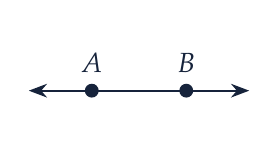
\begin{tikzpicture}\draw[thick,fink,{Stealth}-{Stealth}] (-1.4,0) -- (1.4,0);\fill[fink] (-0.6,0) circle (2.5pt) node[above=3pt]{$A$} (0.6,0) circle (2.5pt) node[above=3pt]{$B$};\path (-1.2,-0.6) rectangle (1.2,0.8);\end{tikzpicture}\par
{\color{fblue}\bfseries Line} $AB$\par\small straight, goes on forever\par\color{gray} both ways: two arrows
\end{column}\pause
\begin{column}{0.31\textwidth}\centering
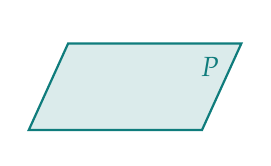
\begin{tikzpicture}\filldraw[fteal!15,draw=fteal,thick] (-1.3,-0.5) -- (0.9,-0.5) -- (1.4,0.6) -- (-0.8,0.6) -- cycle;\node[fteal] at (1.0,0.3){$P$};\path (-1.2,-0.6) rectangle (1.2,0.8);\end{tikzpicture}\par
{\color{fblue}\bfseries Plane} $P$\par\small flat surface, forever\par\color{gray} a floor that never ends
\end{column}
\end{columns}
\end{frame}

\newcommand{\termrow}[4]{\noindent\begin{minipage}[c]{0.17\linewidth}\bfseries\color{fblue} #1\end{minipage}\begin{minipage}[c]{0.31\linewidth}\centering #2\end{minipage}\begin{minipage}[c]{0.14\linewidth}\centering\Large #3\end{minipage}\hfill\begin{minipage}[c]{0.36\linewidth}\small #4\end{minipage}\par}
\begin{frame}{Defined terms --- and their symbols}
\vspace{4pt}
\onslide<1->{\termrow{Line}{\tikz{\draw[thick,{Stealth}-{Stealth}] (0,0)--(2.8,0);\fill (0.6,0) circle(2pt) node[above]{\small$A$} (2.2,0) circle(2pt) node[above]{\small$B$};}}{$\overleftrightarrow{AB}$}{two arrows: goes on forever both ways}}\par\vspace{14pt}
\onslide<2->{\termrow{Ray}{\tikz{\draw[thick,-{Stealth}] (0.6,0)--(2.8,0);\fill (0.6,0) circle(2pt) node[above]{\small$A$} (2.2,0) circle(2pt) node[above]{\small$B$};}}{$\overrightarrow{AB}$}{starts at $A$ --- endpoint written \key{first}}}\par\vspace{14pt}
\onslide<3->{\termrow{Segment}{\tikz{\draw[thick] (0.6,0)--(2.2,0);\fill (0.6,0) circle(2pt) node[above]{\small$A$} (2.2,0) circle(2pt) node[above]{\small$B$};}}{$\overline{AB}$}{two endpoints --- can be measured}}
\end{frame}

\begin{frame}{Length and angle}
\vspace{4pt}
\onslide<1->{\termrow{Length}{\small\color{gray} a number, like $5$ cm}{$AB$}{no bar = the \key{length} of $\overline{AB}$}}\par\bigskip
\onslide<2->{\termrow{Angle}{\tikz[scale=0.8]{\draw[thick,-{Stealth}] (0.6,0)--(3,0);\draw[thick,-{Stealth}] (0.6,0)--(2.4,1.1);\fill (0.6,0) circle(2pt) node[below]{\small$B$} (1.9,0.8) circle(2pt) node[above]{\small$A$} (2.3,0) circle(2pt) node[below]{\small$C$};}}{$\angle ABC$}{vertex $B$ goes in the \key{middle}}}
\end{frame}

\begin{frame}{The mistake almost everyone makes}
\begin{columns}[c]
\begin{column}{0.48\textwidth}\centering
\tikz{\draw[very thick,fteal,-{Stealth}] (0,0)--(3.6,0);\fill (0,0) circle(2.5pt) node[above]{$A$} (2,0) circle(2.5pt) node[above]{$B$};}\par\medskip $\overrightarrow{AB}$ starts at $A$\par\bigskip
\tikz{\draw[very thick,fgold,-{Stealth}] (2,0)--(-1.6,0);\fill (0,0) circle(2.5pt) node[above]{$A$} (2,0) circle(2.5pt) node[above]{$B$};}\par\medskip $\overrightarrow{BA}$ starts at $B$
\end{column}
\begin{column}{0.48\textwidth}
\pause
\warn{$\overrightarrow{AB}$ and $\overrightarrow{BA}$ are \textbf{different} rays --- they start at different points.}\par\medskip\pause
\defn{But $\overline{AB}$ and $\overline{BA}$ are the \textbf{same} segment.}
\end{column}
\end{columns}
\end{frame}

\begin{frame}{Collinear, coplanar, intersection}
\begin{itemize}\setlength\itemsep{14pt}
\item<1-> \key{Collinear}: points on the \textbf{same line}.
\item<2-> \key{Coplanar}: points on the \textbf{same plane}.
\item<3-> Two lines \key{intersect} in a \textbf{point}.\quad
 \tikz[baseline=-3pt]{\draw[thick] (-0.8,-0.4)--(0.8,0.4) (-0.8,0.4)--(0.8,-0.4);\fill[fred] (0,0) circle(2.5pt);}
\item<4-> Two planes \key{intersect} in a \textbf{line}.\quad
 \tikz[baseline=0pt,scale=0.6]{\filldraw[fteal!15,draw=fteal] (-1.6,-0.5)--(1.2,-0.5)--(1.6,0.6)--(-1.2,0.6)--cycle;\filldraw[fgold!20,draw=fgold,opacity=.8] (-0.2,-1)--(0.2,-1)--(0.2,1.2)--(-0.2,1.2)--cycle;\draw[fred,very thick](0,-0.5)--(0,0.6);}
\end{itemize}
\end{frame}

\begin{frame}{}
\begin{yourturn}
Name this figure with the right symbol.\par\medskip
\centering\tikz{\draw[very thick,-{Stealth}] (0,0)--(4.4,0);\fill (0,0) circle(2.5pt) node[above]{$P$} (2.4,0) circle(2.5pt) node[above]{$Q$};}
\end{yourturn}
\pause\bigskip
\centering Answer: \ans{\overrightarrow{PQ}}\quad {\small a ray --- endpoint $P$ first}
\end{frame}

\closeframe{\begin{itemize}\setlength\itemsep{10pt}
\item \key{Line} $\overleftrightarrow{AB}$: two arrows.\quad \key{Ray} $\overrightarrow{AB}$: one arrow, endpoint first.
\item \key{Segment} $\overline{AB}$: a bar.\quad \key{Length} $AB$: no bar --- a number.
\item \key{Angle} $\angle ABC$: the vertex in the middle.
\end{itemize}}
\end{document}
